\documentclass[a4paper,12pt]{jarticle}
\usepackage{url}
\usepackage[dvipdfmx]{graphicx}
\usepackage{epsfig}
\usepackage{amsmath}
\usepackage{amssymb}
\usepackage{times}
\usepackage{ascmac}
\usepackage{here}
\usepackage{txfonts}
\usepackage{listings}

\renewcommand{\lstlistingname}{リスト}
\lstset{language=Perl,
  basicstyle=\ttfamily\scriptsize,
  commentstyle=\textit,
  classoffset=1,
  keywordstyle=\bfseries,
  frame=tRBl,
  framesep=5pt,
  showstringspaces=false,
  numbers=left,
  stepnumber=1,
  numberstyle=\tiny,
  tabsize=2
}

 \lstdefinelanguage{CASL2}{
   morekeywords={C, C++, Ruby},
   morecomment=[l]{;},
   morestring=[b]",%"
 }

\setlength{\oddsidemargin}{-.2in}
\setlength{\evensidemargin}{-.2in}
\setlength{\topmargin}{-4em}
\setlength{\textwidth}{6.5in}
\setlength{\textheight}{10in}
\setlength{\parskip}{0em}
\setlength{\topsep}{0em}
\setlength{\columnsep}{3zw}

\title{シミュレーション物理 5}
\author{200911434 青木大祐}

\begin{document}
\maketitle
\newpage

\section{演習問題10}
実験に用いたソースコードを以下に示す。

\begin{lstlisting}
use v6;
constant M = 1;
constant H = 3.5;
constant $nm = 99;

class Planet {
    has $.x_pos is rw;
    has $.y_pos is rw;
    has $.x_spd;
    has $.y_spd;

    method new {
        my $x_pos;
        my $y_pos;
        loop {
            $x_pos = 2.rand - 1;
            $y_pos = 2.rand - 1;
            last if $x_pos.abs ** 2 + $y_pos.abs ** 2 < 4;
        }

        self.bless(*, x_pos => $x_pos + ($nm + 1)/2 , y_pos => $y_pos + ($nm + 1)/2,
               x_spd => $x_pos, y_spd => $y_pos);
    }

    method next_pos (@Fx) {
        my %Fp;
        %Fp<F> = @Fx[$.x_pos + 0.5][$.y_pos + 0.5];
        my $dx = (($.x_pos + 0.5).floor - $.x_pos).abs;
        my $dy = (($.y_pos + 0.5).floor - $.y_pos).abs;
        %Fp<x> = M * %Fp<F> * ($dx / ($dx + $dy));
        %Fp<_y> = M * %Fp<F> * ($dy  / ($dx + $dy));
        $.x_pos += ($.x_spd + (%Fp<x> / M) * 0.1) * 0.1;
        $.y_pos += ($.y_spd + (%Fp<y> / M) * 0.1) * 0.1;
        return self;
    }
}


my $ni = 50;
my $G = 1;
my $dx = 1;

my Planet @ps;
@ps.push(Planet.new) for ^500;
dump("./before.csv", @ps);

my @tmp;
@tmp.push([0 xx $nm+1]) for ^($nm+1);

for ^41 {
    say $_;
    my @phi = @tmp;
    my @ro = @tmp;
    my @Fx = @tmp;
    for @ps {
        @ro[.x_pos + 0.5][.y_pos + 0.5] += 1 ;
    }

    say @ro.map({.gist ~ "\n"});
    calc(@phi, $nm, $ni, $G, $dx, @ro);

    for 0..^$nm X 0..^$nm -> $x, $y {
        @Fx[$x][$y] = - (@phi[$x + 1][$y] - @phi[$x][$y])/$dx;
    }

    @ps.=map(*.next_pos(@Fx));
    dump($_ ~ ".csv", @ps) if $_ == 0|20|40;
    last; #
}

sub dump (Str $fname, @ps) {

    my $file = open $fname, :w;
    for @ps {
        $file.say(($_.x_pos, $_.y_pos).join(","))
    }
    $file.close
}

sub calc (@phi is rw, $nm, $ni, $G, $dx, @ro) {
    for ^$ni {
        for 1..^$nm X 1..$^nm -> $ix, $iy {
            my $p1 = @phi[$ix+1][$iy] + @phi[$ix-1][$iy] + @phi[$ix][$iy+1] + @phi[$ix][$iy-1];
            my $p2 = $G * @ro[$ix][$iy] * $dx * $dx;
            @phi[$ix][$iy] = ($p1/4) - ($p2/4);
        }
    }
}

\end{lstlisting}
\vspace{4zh}
\section{実行結果}
以下に、nk = 0, 20, 40の散布図を示す。
\center
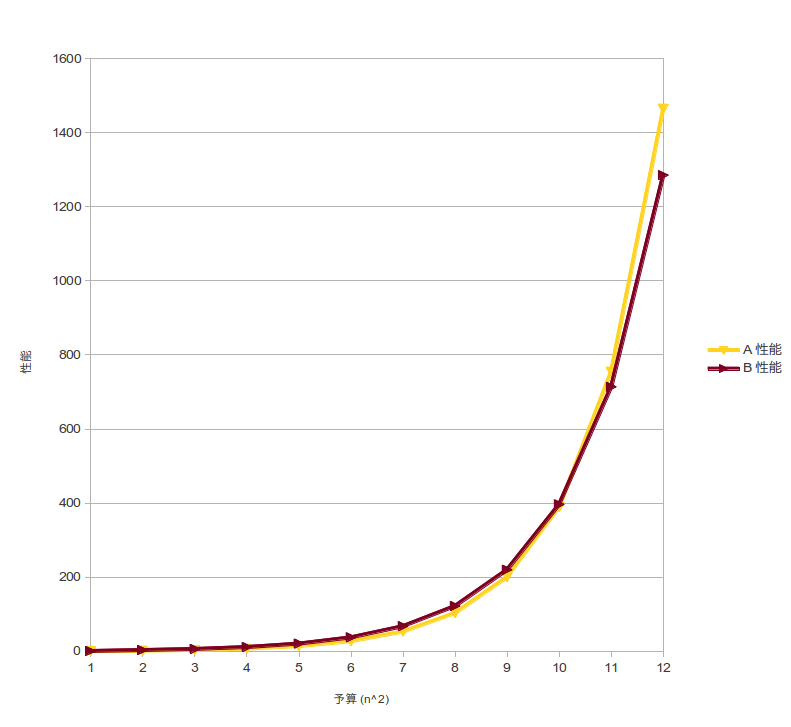
\includegraphics[width=10cm]{graph.png}
\end{document}